\documentclass[../document.tex]{subfiles}

\begin{document}
    \subsection{Индивидуальное задание практики}
    \par В качестве индивидуального задания практики было поручено исследовать возможность распознавания медведей при помощи методов машинного обучения.
    \par Само по себе распознавание медведей является актуальной и интересной задачей, так как разработанные решения можно использовать для:
    \begin{itemize}
    	\item Исследование поведения медведей
    	\item Обеспечение безопасного проведения работ в областях, которые расположены в местах обитания медведей
    	\item Исследование миграции медведей
    	\item Наблюдение за медведями в местах их содержания(вольеры, заповедники и т.д.)
    \end{itemize}
    
    \subsection{Выбор моделей}
	    \par Для выполнения задания в первую очередь требовалось выбрать рассматриваемые модели. К моделям были применены следующие требования, а именно:
	    \begin{itemize}
	    	\item Быстродействие
	    	\item Точность
	    	\item Возможность решать задачи классификации изображений или детекции
	    \end{itemize}
	    \par В частном случае задача детекции была превращена в задачу классификации, так как если модель смогла на изображении найти объект с нужным классом, то в качестве ответа получали только метку класса, а именно есть медведь на изображении или он отсутствует.
	    \par Были выбраны следующие модели:
	    \begin{itemize}
	    	\item YOLO
	    	\item RT-DETR
	    	\item Faster R-CNN
	    \end{itemize}
	    \par Для всех моделей были использованы веса, которые обучили на датасете Common Objects in Context (COCO).
    
    \subsection{YOLO}
	    \par Когда в задаче говорится о детекции объектов, то в первую очередь для решения этой задачи в голову приходит архитектура YOLO.
	    \par YOLO (You Only Look Once), популярная модель обнаружения объектов и сегментации изображений, была разработана Джозефом Редмоном и Али Фархади в Университете Вашингтона. Появившись в 2015 году, YOLO быстро завоевала популярность благодаря своей высокой скорости и точности.
	    \par На сегодняшний день существует не менее 10 версий описываемой архитектуры.
	    \par Алгоритм YOLO, был первой попыткой сделать возможной детекцию объектов в реальном времени. В рамках алгоритма YOLO исходное изображение сначала разбивается на сетку из $N×N$ ячеек. Если центр объекта попадает внутрь координат ячейки, то эта ячейка считается ответственной за определение параметров местонахождения объекта. Каждая ячейка описывает несколько вариантов местоположения ограничивающих рамок для одного и того же объекта. Каждый из этих вариантов характеризуется пятью значениями — координатами центра ограничивающей рамки, его шириной и высотой, а также степени уверенности в том, что ограничивающая рамка содержит в себе объект. Также необходимо для каждой пары класса объектов и ячейки определить вероятность того, что ячейка содержит в себе объект этого класса. Таким образом, последний слой сети, принимающий конечное решение об ограничивающих рамках и классификации объектов работает с тензором размерности $N×N×(5B+C)$, где $B$ — количество предсказываемых ограничивающих рамок для ячейки, $C$ — количество классов объектов, определённых изначально.
	    
	    \begin{figure}[H]
	    	\centering
	    	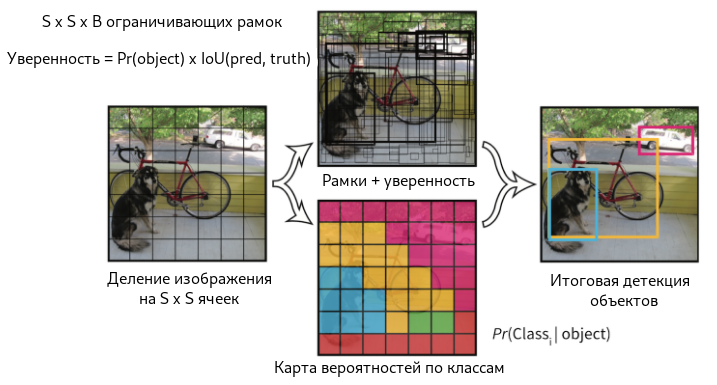
\includegraphics[scale=0.5]{YOLO_alg.png}
	    	\caption{Алгоритм YOLO}
	    \end{figure}
	    \begin{figure}[H]
	    	\centering
	    	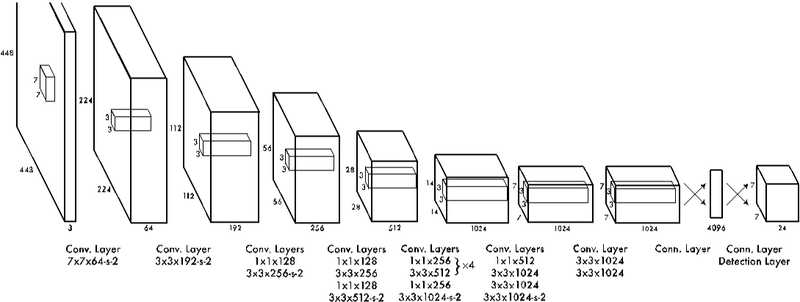
\includegraphics[scale=0.5]{YOLO_arch.png}
	    	\caption{Архитектура YOLO}
		\end{figure}
	
	\subsection{RT-DETR}
		\par Следующей исследуемой архитектурой стали визуальные трансформеры. К использованию Real-Time Detection Transformer(RT-DETR) подтолкнула статья на arxiv "DETRs Beat YOLOs on Real-time Object Detection" и готовая реализация в бибилотеке ultralytics.
		\par По мению авторов статьи, использование подавления немаксимумов (Non-Maximum Suppression, NMS), который является важных шагом в детекции YOLO, негативно сказывается на производительности и точности модели. В свою очередь авторы отказываюстя от NMS и описывают свою архитектуру следующим образом.
		\par Мы передаем признаки из последних трех слоев бэкбона в кодер. Эффективный гибридный кодер преобразует многомасштабные признаки в последовательность признаков изображения посредством внутримасштабного взаимодействия признаков основанного на внимании (Attention based Intra-scale Feature Interaction, AIFI) и слияния межмасштабных признаков на основе CNN (CNN-based Cross-scale Feature Fusion, CCFF). Затем выбор запроса с минимальной неопределенностью выбирает фиксированное количество признаков кодера, которые будут служить начальными объектными запросами для декодера. Наконец, декодер со вспомогательными головами прогнозирования итеративно оптимизирует объектные запросы для генерации категорий и блоков.
		\begin{figure}[H]
			\centering
			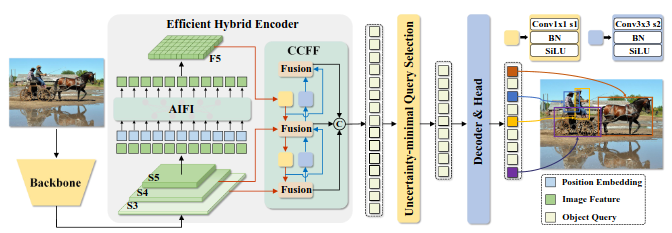
\includegraphics[scale=0.5]{RT-DETR_arch.png}
			\caption{Представление RT-DETR}
		\end{figure}
		
		\par Также авторы сделали бенчмарк с датасетом MS COCO и сравнили свою архитектуру с другими моделями детекции в реальном времени и показали, что их архитектура достигает SOTA
		\begin{figure}[H]
			\centering
			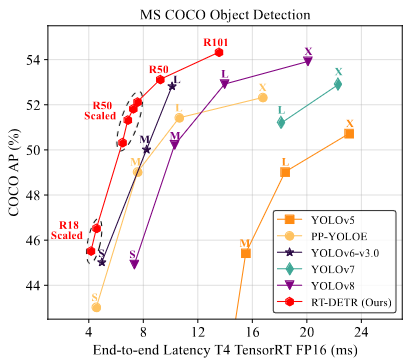
\includegraphics[scale=0.5]{RT-DETR_test.png}
			\caption{Сравнение RT-DETR с другими моделями детекции}
		\end{figure}
	
	\subsection{Faster R-CNN}
		\par Заключительной рассматриваемой архитектурой стали Сверточные сети, основанные на регионах
 или же Region-based CNN (R-CNN), а в частности их модификация Faster R-CNN.
 		\par Эта архитектура была выбрана для рассмотрения как одна из классических архитектур, которая решает задачу детекции. В её основе лежит алгоритм выборочного поиска (Selective Search). Данный алгоритм получает на вход изображение, а на выходе выдает массив прямоугольников, в которых возможно находится объект. И идея такова, что в первую очередь будет проведен выборочный поиск, при помощи которого мы получим кропы изображений, а уже эти кропы мы помещаем в классификатор.
 		\par В дальнейшем эту идею развили, потому что нам не нравилось, что для каждой гипотезы из выборочного поиска мы выполняли классификацию, поэтмоу решили сперва выполнить свертку и получить карту признаков(Feature Map), затем на исходном изображении получить гипотезы и их спроецировать на карту признаков. Этот алгоритм назвали Fast R-CNN.
 		\par Заключительной идее в R-CNN стало следующее: выборочный поиск решили заменить на нейронную сеть. И теперь поиск границ объектов это тоже обучаемый алгоритм.
 		
 		\begin{figure}[H]
 			\centering
 			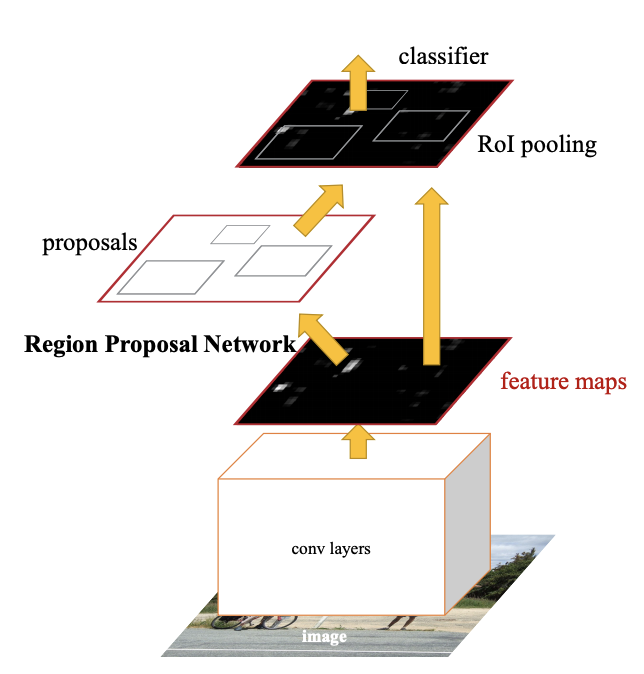
\includegraphics[scale=0.5]{R-CNN_alg.png}
 			\caption{Принцип работы Faster R-CNN}
 		\end{figure}
 		
\end{document}
